\documentclass[11pt,preprint, authoryear]{elsarticle}

\makeatletter
\renewcommand\@biblabel[1]{}
\makeatother

\usepackage{lmodern}
%%%% My spacing
\usepackage{setspace}
\setstretch{1.2}
\DeclareMathSizes{12}{14}{10}{10}

% Wrap around which gives all figures included the [H] command, or places it "here". This can be tedious to code in Rmarkdown.
\usepackage{float}
\let\origfigure\figure
\let\endorigfigure\endfigure
\renewenvironment{figure}[1][2] {
    \expandafter\origfigure\expandafter[H]
} {
    \endorigfigure
}

\let\origtable\table
\let\endorigtable\endtable
\renewenvironment{table}[1][2] {
    \expandafter\origtable\expandafter[H]
} {
    \endorigtable
}


\usepackage{ifxetex,ifluatex}
\usepackage{fixltx2e} % provides \textsubscript
\ifnum 0\ifxetex 1\fi\ifluatex 1\fi=0 % if pdftex
  \usepackage[T1]{fontenc}
  \usepackage[utf8]{inputenc}
\else % if luatex or xelatex
  \ifxetex
    \usepackage{mathspec}
    \usepackage{xltxtra,xunicode}
  \else
    \usepackage{fontspec}
  \fi
  \defaultfontfeatures{Mapping=tex-text,Scale=MatchLowercase}
  \newcommand{\euro}{€}
\fi

\usepackage{amssymb, amsmath, amsthm, amsfonts}

\def\bibsection{\section*{References}} %%% Make "References" appear before bibliography


\usepackage[round]{natbib}

\usepackage{longtable}
\usepackage[margin=2.3cm,bottom=2cm,top=2.5cm, includefoot]{geometry}
\usepackage{fancyhdr}
\usepackage[bottom, hang, flushmargin]{footmisc}
\usepackage{graphicx}
\numberwithin{equation}{section}
\numberwithin{figure}{section}
\numberwithin{table}{section}
\setlength{\parindent}{0cm}
\setlength{\parskip}{1.3ex plus 0.5ex minus 0.3ex}
\usepackage{textcomp}
\renewcommand{\headrulewidth}{0.2pt}
\renewcommand{\footrulewidth}{0.3pt}

\usepackage{array}
\newcolumntype{x}[1]{>{\centering\arraybackslash\hspace{0pt}}p{#1}}

%%%%  Remove the "preprint submitted to" part. Don't worry about this either, it just looks better without it:
\makeatletter
\def\ps@pprintTitle{%
  \let\@oddhead\@empty
  \let\@evenhead\@empty
  \let\@oddfoot\@empty
  \let\@evenfoot\@oddfoot
}
\makeatother

 \def\tightlist{} % This allows for subbullets!

\usepackage{hyperref}
\hypersetup{breaklinks=true,
            bookmarks=true,
            colorlinks=true,
            citecolor=blue,
            urlcolor=blue,
            linkcolor=blue,
            pdfborder={0 0 0}}


% The following packages allow huxtable to work:
\usepackage{siunitx}
\usepackage{multirow}
\usepackage{hhline}
\usepackage{calc}
\usepackage{tabularx}
\usepackage{booktabs}
\usepackage{caption}


\newenvironment{columns}[1][]{}{}

\newenvironment{column}[1]{\begin{minipage}{#1}\ignorespaces}{%
\end{minipage}
\ifhmode\unskip\fi
\aftergroup\useignorespacesandallpars}

\def\useignorespacesandallpars#1\ignorespaces\fi{%
#1\fi\ignorespacesandallpars}

\makeatletter
\def\ignorespacesandallpars{%
  \@ifnextchar\par
    {\expandafter\ignorespacesandallpars\@gobble}%
    {}%
}
\makeatother

\newlength{\cslhangindent}
\setlength{\cslhangindent}{1.5em}
\newenvironment{CSLReferences}%
  {\setlength{\parindent}{3pt}%
  \everypar{\setlength{\hangindent}{\cslhangindent}}\ignorespaces}%
  {\par}


\urlstyle{same}  % don't use monospace font for urls
\setlength{\parindent}{0pt}
\setlength{\parskip}{6pt plus 2pt minus 1pt}
\setlength{\emergencystretch}{3em}  % prevent overfull lines
\setcounter{secnumdepth}{5}

%%% Use protect on footnotes to avoid problems with footnotes in titles
\let\rmarkdownfootnote\footnote%
\def\footnote{\protect\rmarkdownfootnote}
\IfFileExists{upquote.sty}{\usepackage{upquote}}{}

%%% Include extra packages specified by user

%%% Hard setting column skips for reports - this ensures greater consistency and control over the length settings in the document.
%% page layout
%% paragraphs
\setlength{\baselineskip}{12pt plus 0pt minus 0pt}
\setlength{\parskip}{12pt plus 0pt minus 0pt}
\setlength{\parindent}{0pt plus 0pt minus 0pt}
%% floats
\setlength{\floatsep}{12pt plus 0 pt minus 0pt}
\setlength{\textfloatsep}{20pt plus 0pt minus 0pt}
\setlength{\intextsep}{14pt plus 0pt minus 0pt}
\setlength{\dbltextfloatsep}{20pt plus 0pt minus 0pt}
\setlength{\dblfloatsep}{14pt plus 0pt minus 0pt}
%% maths
\setlength{\abovedisplayskip}{12pt plus 0pt minus 0pt}
\setlength{\belowdisplayskip}{12pt plus 0pt minus 0pt}
%% lists
\setlength{\topsep}{10pt plus 0pt minus 0pt}
\setlength{\partopsep}{3pt plus 0pt minus 0pt}
\setlength{\itemsep}{5pt plus 0pt minus 0pt}
\setlength{\labelsep}{8mm plus 0mm minus 0mm}
\setlength{\parsep}{\the\parskip}
\setlength{\listparindent}{\the\parindent}
%% verbatim
\setlength{\fboxsep}{5pt plus 0pt minus 0pt}



\begin{document}



%titlepage
\thispagestyle{empty}
\begin{center}
\begin{minipage}{0.75\linewidth}
    \centering
%Entry1
    {\uppercase{\huge A Game Theoretic Approach to Deadline
Adherence\par}}
    \vspace{2cm}
%Author's name
    {\LARGE Microeconomics 871 Essay\par}
    \vspace{1cm}
%University logo
\begin{center}
    
\includegraphics[width=0.6\linewidth]{Tex/deadline.png}
\end{center}
\vspace{1cm}
%Supervisor's Details
\begin{center}
    {\LARGE \textbf{Jessica van der Berg - 20190565}\par}
    \vspace{1cm}
%Degree
    {\LARGE \textbf{Laura Meyer - 20748302}\par}
    \vspace{1cm}
%Institution
    {\LARGE \textbf{Cassandra Pengelly - 20346212}\par}
    \vspace{1cm}
%Date
    {\large 18 October 2021 \textbar{} Word Count: 1998}
%More
    {\normalsize }
%More
    {\normalsize }
\end{center}
\end{minipage}
\end{center}
\clearpage


\begin{frontmatter}  %

\title{}

% Set to FALSE if wanting to remove title (for submission)


\vspace{1cm}





\vspace{0.5cm}

\end{frontmatter}


\renewcommand{\contentsname}{Table of Contents}
{\tableofcontents}

%________________________
% Header and Footers
%%%%%%%%%%%%%%%%%%%%%%%%%%%%%%%%%
\pagestyle{fancy}
\chead{}
\rhead{}
\lfoot{}
\rfoot{\footnotesize Page \thepage}
\lhead{}
%\rfoot{\footnotesize Page \thepage } % "e.g. Page 2"
\cfoot{}

%\setlength\headheight{30pt}
%%%%%%%%%%%%%%%%%%%%%%%%%%%%%%%%%
%________________________

\headsep 35pt % So that header does not go over title




\newpage

\hypertarget{introduction}{%
\section{\texorpdfstring{Introduction
\label{intro}}{Introduction }}\label{introduction}}

Various theories of the relationship between lecturer and student show
that a student's actions are often influenced by the behaviour of their
lecturer (\protect\hyperlink{ref-power}{Conrad, 1983}),
(\protect\hyperlink{ref-comm}{Conrad, 1991}),
(\protect\hyperlink{ref-trust}{Liu \& Shi, 2017}). Identity-based
motivation theory posits that a relationship of trust and leniency
between student and lecturer causes both to better reach their goals,
increases performance, and improves mental health
(\protect\hyperlink{ref-trust}{Liu \& Shi, 2017}). Lecturers often
require students to complete tasks, including essays, before a deadline.
Game theoretic models provide a useful framework to analyse the
interactions between a student and lecturer
(\protect\hyperlink{ref-book}{Osborne, 2004}) since they offer insights
into when a student may choose to miss a deadline and when a lecturer
will give an extension, in the presence of incomplete information.

The paper considers the strategic interaction of students and lecturers
in the context of dynamic games of incomplete information. A student is
required to submit an assignment with by a certain deadline, but
experiences a crisis and must choose whether to hand in either on time
or late. Both players have continuous type spaces and a discrete set of
actions.

The remainder of the essay\footnote{This essay was written in R using
  the package Texevier by \protect\hyperlink{ref-Texevier}{Katzke}
  (\protect\hyperlink{ref-Texevier}{2017}). \newline The code for this
  essay can be found on Github
  \href{https://github.com/cass-code/Essay}{here.}} is organised as
follows. section \ref{lit} discusses the literature on games of
incomplete information with applications. Section \ref{game} presents
our model of deadline adherence. Section \ref{result} analyses the
solutions to the game. Section \ref{extension} provides an extension of
the game and the final section \ref{con} concludes.

\hypertarget{games-of-incomplete-information}{%
\section{\texorpdfstring{Games of Incomplete Information
\label{lit}}{Games of Incomplete Information }}\label{games-of-incomplete-information}}

When making decisions, agents often do not have full information
(\protect\hyperlink{ref-2020games}{Trabelsi, 2020}).
\protect\hyperlink{ref-von}{Von Neumann \& Morgenstern}
(\protect\hyperlink{ref-von}{1944: 30}) first used the term
\emph{incomplete information} to describe a model in which parts of the
normal form structure was unspecified. However, Von Neumann and
Morgenstern deemed further research into such a model unimportant
(\protect\hyperlink{ref-2004com}{Myerson, 2004}).
\protect\hyperlink{ref-luce1956}{Luce \& Adams}
(\protect\hyperlink{ref-luce1956}{1956}) disagreed and extended on the
incomplete information literature by assuming that each player has a
perception of the payoff function of the other player. A player's
perception does not have be a true reflection of the other player's
payoffs, but it forms the basis of the player's strategy.
\protect\hyperlink{ref-harsanyi}{Harsanyi}
(\protect\hyperlink{ref-harsanyi}{1995}) developed a general analytical
framework for games of incomplete information, which made it practical
to solve the games.

Following Harsanyi's approach, players have less than full information
about each others payoff functions and, based on Bayesian methodology,
both players have expectations in the form of subjective probability
distributions (\protect\hyperlink{ref-harsanyi}{Harsanyi, 1995}). Both
players estimate the probability that the other player is of a certain
type, subject to the available information. To solve the model, the game
of incomplete information will be reinterpreted as a game with complete
and imperfect information, through transforming its basic mathematical
structure by adding nature as a third player.

\hypertarget{a-model-of-deadline-adherence}{%
\section{\texorpdfstring{A Model of Deadline Adherence
\label{game}}{A Model of Deadline Adherence }}\label{a-model-of-deadline-adherence}}

The model of deadline adherence sheds some light on how students think
about assignment submissions, and how lecturers respond when assignments
are submitted late. In the model, a student receives an assignment with
a due date set by the lecturer. While the student is working on the
assignment, she experiences a crisis and therefore spends less time on
the assignment. She has two options: she can hand in the assignment on
time or she can hand in late. If she hands in on time, she will get a
payoff of \(a-c\), where \(a\) is her potential pre-crisis mark, and
\(c\) is the negative academic impact of the crisis. Submitting late
gives the student the opportunity to recover some of the cost of the
crisis on her final mark. If the lecturer gives her a penalty for late
submission, her payoff is \(a-\beta c -m\), where \(m\) is the
percentage point penalty subtracted from her final mark. If the lecturer
decides the waive the penalty, the student gets a payoff of
\(a-\beta c\). The parameter \(\beta \in [0,1]\) represents the type of
the student. A low \(\beta\) suggests a strong academic resiliency,
whereas a high \(\beta\) suggests low resiliency. The student observes
her own type but not the lecturer's type.

The lecturer decides whether to give a penalty, \(m\), if a student
submits late. The lecturer has disutility from giving a penalty since
the student submitted late due to a crisis. The magnitude of her
disutility depends on the magnitude of the penalty, \(m\), and the
lecturer's degree of empathy. The parameter \(\delta \in [0,1]\) denotes
the lecturer's penalty, describing her type. A higher \(\delta\) implies
that a lecturer is more empathetic. The lecturer observes her own type
but not the student's type. If the lecturer does not impose a penalty,
he derives benefit from helping a student through a difficult time
academically, yielding the payoff \(\delta c\). The lecturer knows that
by waiving the penalty, he may be encouraging this student, and other
students to hand in late in the future. The lecturer would rather deter
late hand-ins, and receives a negative payoff \(d\) for not
deterring\footnote{This deterrent parameter relates to the literature on
  games of repeated interaction and reputations
  (\protect\hyperlink{ref-deter}{Clark \& Montgomery, 1998}).} late
hand-ins.

The lecturer and student both have continuous type spaces, which are
assumed to be independently and randomly chosen by nature at the start
of the game from a uniform distribution\footnote{A uniform distribution
  puts equal chance on any of the outcomes between 0 and 1 happening.
  Other, more realistic, probability distributions have been omitted for
  ease of interpretation. Assuming a normal distribution would give a
  similar interpretation of how changes in parameters affect the
  outcomes but would needlessly complicate the game.}:
\(\delta \sim Uniform(0,1)\) and \(\beta \sim Uniform(0,1)\). The
parameters \(a,\, c,\, m\, \&\, d\) are all common knowledge. Each
player needs to choose his/her action based on his/her own type, their
beliefs of the other player's type, and the values of parameters
\(a,\, c,\, m\, \&\, d\). Figure \ref{Figure1} shows the game in
extensive form\footnote{The simultaneous form game can be found in the
  appendix \ref{tab1}} and figure \ref{sum} shows a summary of the
game's parameters.

\begin{center}
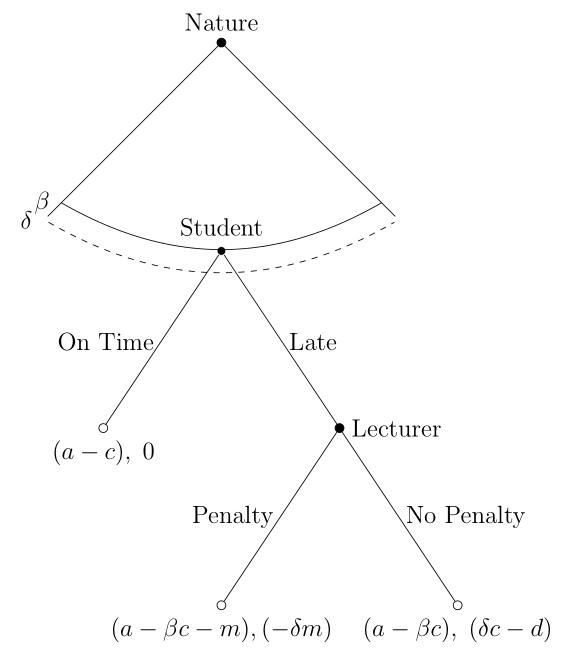
\includegraphics[scale=1]{"img/continuous.jpg"}
\captionof{figure}{This game is dynamic, where nature first chooses the student's and lecturer's types. The dashed line represents information only known by the lecturer and the solid line represents information only known by the student. Then the student moves, deciding to hand in on time or late after experiencing a crisis. If the student hands in late, the lecturer decides to impose a penalty or not. }
\label{Figure1}
\end{center}

\begin{table}[H]
\centering
\begin{tabular}{lll}
  \toprule
Parameter & Explanation & Restriction \\ 
  \midrule
$a$ & Potential assignment mark & $0\leq a \leq 1$ \\ 
  $c$ & Cost of crisis to assignment mark & $0 < c \leq 1$ \\ 
  $\beta$ & Student's type: level of resiliency & $\beta \sim Uniform(0,1)$  \\ 
  $m$ & Mark penalty & $0 < m \leq 1$ \\ 
  $\delta$ & Lecturer's type: level of empathy & $\delta \sim Uniform(0,1)$ \\ 
  $d$ & Detterent & $0<d \leq 1$ \\ 
   \bottomrule
\end{tabular}
\caption{Game Parameters \label{sum}} 
\end{table}

\hypertarget{results-and-discussion}{%
\section{\texorpdfstring{Results and Discussion
\label{result}}{Results and Discussion }}\label{results-and-discussion}}

We solve for the players' best responses to understand how the lecturer
and student will make their decisions given their beliefs. The best
response for the student would be to hand in on time if the expected
payoff from handing in on time is higher than the expected payoff of
submitting late. Defining \(p\) as the probability that the lecturer
will give a penalty, a student should hand in on time where:\\
\begin{align*}
\beta>\frac{c-m p}{c}
\end{align*} The right hand side is a constant\footnote{Since \(c\) and
  \(m\) are known, and \(p\) is a belief the student holds.}. This
implies that there is some threshold value of \(\beta\), for which a
student should hand in on time. If the student believes that the
lecturer will give no penalty (i.e.~\(p=0\)), then she should only hand
in on time if \(\beta > \frac{c}{c} \Rightarrow \beta > 1\). Since
\(\beta\) lies between \(0\) and \(1\), the inequality will never hold
and she should always hand in late. Intuitively, a student can never do
worse by handing in late if there is no penalty\footnote{Handing in late
  is a weakly dominant strategy.} but she will do better to hand in late
if she is resilient in any way (\(\beta < 1\)) and can partially recover
from the crisis.

However, if the student believes that the lecturer will give a penalty
with some positive probability (\(p>0\)) then her decision to hand in on
time depends on her level of resiliency, the magnitude of the crisis and
the size of the penalty. As the cost of the crisis increases, the
threshold value increases and the student becomes more likely to hand in
late, unless her she has a very low resiliency. If the mark penalty is
high, the threshold value is smaller and the student is more likely to
hand in on time, unless she is very resilient (i.e., \(\beta\) is very
low). We analyse the lecturer's best response rule similarly. The
lecturer should impose a penalty where: \begin{align*}
\delta<\frac{d}{c+m}
\end{align*} The threshold value for the lecturer is the ratio between
the deterrent factor and the sum of the cost of the crisis and the
penalty mark. If the deterrent factor is high relative to the cost of
crisis and the penalty mark, then the lecturer is more likely to give a
penalty. If the cost of the crisis large and the mark penalty is high
relative to the deterrent factor, the lecturer is more likely to give no
penalty. A highly empathetic lecturer is more likely to waive the
penalty.

While best response analysis is useful, solving for the Bayesian Nash
Equilibrium (BNE) is necessary if one wants to understand the outcome of
the game and the players' strategies. The full derivations of the
solution concepts can be found in the appendix (\ref{B}).

After observing her private type, the student chooses the following
hand-in pattern:\\
\begin{align*}
s_{\beta}^{*}(\beta)=\left\{\begin{array}{lll}
\text{On time} & \text{if} & \beta>1-\frac{m d}{c^{2}+m c}  \\
\text{Late} & \text{if} & \beta \leq 1-\frac{m d}{c^{2}+m c} 
\end{array}\right.
\end{align*}

And the lecturer's BNE strategy is given by: \begin{align*}
s_{\delta}^{*}(\delta)=\left\{\begin{array}{lll}
\text{Penalty} & \text { if } & \delta<\frac{d}{c+m} \\
\text{No penalty} & \text { if } & \delta \geq \frac{d}{c+m}
\end{array}\right.
\end{align*}

When both players play their equilibrium strategies neither has an
incentive to deviate, resulting in a BNE. We would interpret the
student's BNE strategy similarly to her best response, however, her
strategy profile only depends on her own type and no longer on her
beliefs about the lecturer's type. The lecturer's best response function
and equilibrium strategy profile are the same because the lecturer
observes whether the student hands in late or not and therefore has no
need to hold beliefs about when the student will hand in.

\hypertarget{extension}{%
\section{\texorpdfstring{Extension
\label{extension}}{Extension }}\label{extension}}

We extend the game above to account for grade inflation. The lecturer
has an incentive to inflate a student's grade since a higher grade is
associated with a more favourable evaluation from the student.
Favourable evaluations are linked to an increase in salary and a higher
likelihood of promotion for the lecturer
(\protect\hyperlink{ref-2018grades}{Goswami \& Mumit, 2018}). However,
inflating a grade is ethically wrong; therefore, the lecturer incurs a
cost of \(\gamma\) if he decides to inflate. If the lecturer leaves the
mark unchanged, he incurs an empathy cost of \(\delta\). A student
experiences a cost of \(\omega\) for asking the lecturer, and the
lecturer experiences a cost of \(\phi\) for being bothered by the
student. If the lecturer decides not to penalise the student, then he
will never choose to inflate a students mark. Knowing this, a student
that hands in late and receives no penalty will always accept her mark.
If a student hands in on time, a lecturer will always leave the mark
unchanged at the request of the student; therefore the student will
always accept the mark. If the lecturer decides to penalise a late
student, the lecturer will choose to inflate a student's mark given that
the ethical cost is smaller than the empathy cost the lecturer
experiences;\\
\[\gamma < \delta m \] If the ethical cost the lecturer experiences is
larger than the empathy cost, then the lecturer is strict. Otherwise,
the lecturer is lenient. As such, a strict lecturer will not inflate a
student's mark, but a lenient lecture will
(\protect\hyperlink{ref-2010grade}{Franz, 2010}).

A summary of the game's parameters and restrictions are shown in table
\ref{table:ext} and the game is represented in Figure \ref{fig:extd}

\begin{table}
\caption{Extended Game Parameters}
\centering
\begin{tabular}{c c c} \hline
Parameter & Explanation & Restrictions \\
\hline 
\(\omega\) & Exogenous cost of asking for the lecturer for higher mark & 0 < \(\omega\) $\le$ 1 \\
\(\gamma\) & Ethical cost of inflating students mark & 0 < \(\delta\) $\le$ 1 \\
\(\phi\) & Cost of annoyance lecture experience for student bothering him & 0 <\(\phi\) $\le$ 1 \\
x & Additional marks that student get when lecturer decides to inflates &  1 < x $\le$ 2 \\ [1ex]
\hline 
\end{tabular}
\label{table:ext}
\end{table}

\begin{center}
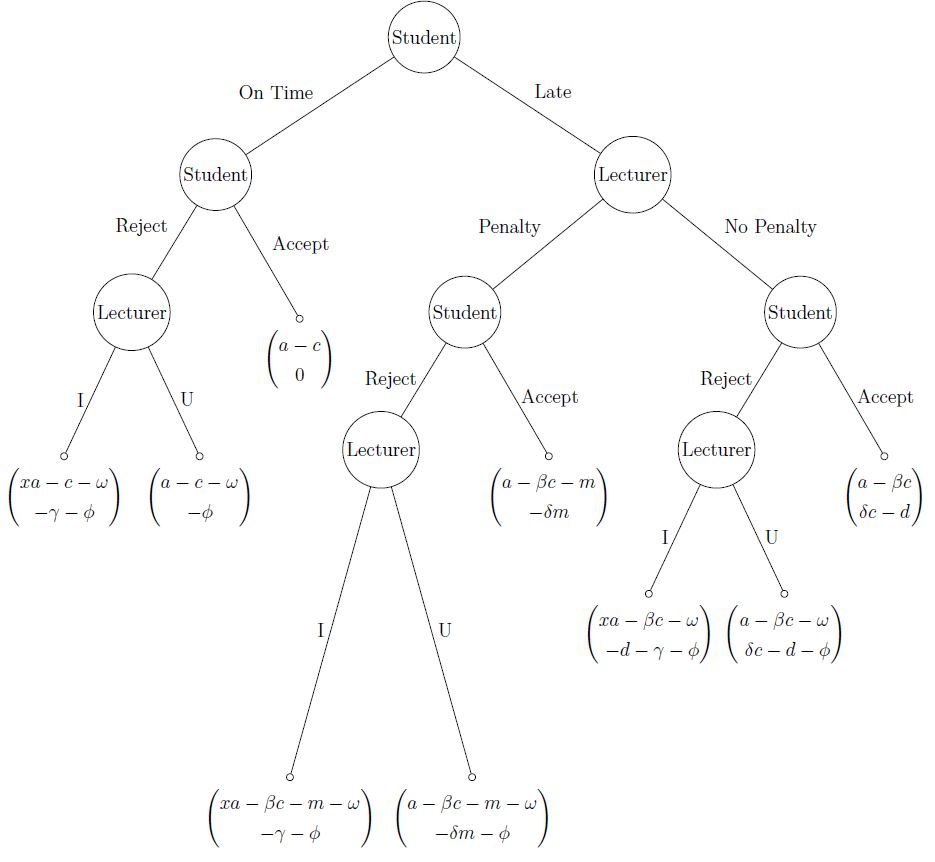
\includegraphics[scale=0.90]{"img/extend.jpg"}
\captionof{figure}{This is an extended version of the game presented in Figure 3.1. To account for grade inflation, the student gets to accept the grade the lecturer game him, or reject the grade and ask the lecturer for a better mark. The lectuerer can then decided to inflate (I) the students mark or leave the mark unchanged (U). }
\label{fig:extd}
\end{center}

\hypertarget{conclusion}{%
\section{\texorpdfstring{Conclusion
\label{con}}{Conclusion }}\label{conclusion}}

The results of the model are intuitive and provide a useful insight into
how students think about handing in assignments, and how lecturers
respond to late submissions. Whether a lecturer penalises a student for
late submission depends largely on the magnitude of the crisis the
student is facing, relative to the lecturer's degree of empathy. The
student chooses whether to hand in late depending on the inconvenience
to the lecturer, the size of the penalty, the magnitude of the crisis,
and their ability to bounce back from an academic setback.

One shortcoming of the model is that it assumes c is common knowledge.
Lecturers often have too many students to have a personal relationship
with each one to know if they are experiencing a crisis. Another
shortcoming is that the lecturer's benefit from giving no penalty does
not account the benefit of no penalty to the student. More resilient
students would fare well to hand in late since they recover from the
crisis easily. However, if the lecturer's decision to penalise a student
also depends on the student's resiliency, it would deter students with
low resiliency from taking an extension, allowing them to focus on their
other work due later in the term.

\newpage

\hypertarget{references}{%
\section*{References}\label{references}}
\addcontentsline{toc}{section}{References}

\hypertarget{refs}{}
\begin{CSLReferences}{1}{0}
\leavevmode\hypertarget{ref-deter}{}%
Clark, B.H. \& Montgomery, D.B. 1998. Deterrence, reputations, and
competitive cognition. \emph{Management Science}. 44(1):62--82.
{[}Online{]}, Available: \url{http://www.jstor.org/stable/2634427}.

\leavevmode\hypertarget{ref-power}{}%
Conrad, C. 1983. Power and performance as correlates of supervisors'
choice of modes of managing conflict: A preliminary investigation.
\emph{Western Journal of Communication (includes Communication
Reports)}. 47(3):218--228.

\leavevmode\hypertarget{ref-comm}{}%
Conrad, C. 1991. Communication in conflict: Style-strategy
relationships. \emph{Communications Monographs}. 58(2):135--155.

\leavevmode\hypertarget{ref-2010grade}{}%
Franz, W.-J.I. 2010. Grade inflation under the threat of students'
nuisance: Theory and evidence. \emph{Economics of Education Review}.
29(3):411--422.

\leavevmode\hypertarget{ref-2018grades}{}%
Goswami, G.G. \& Mumit, A. 2018. Are grades inflated for good teaching
evaluations? Evidence from bangladesh. \emph{Goswami, GG and Mumit,
A.(2018)." Are Grades Inflated for Good Teaching Evaluations}. 203--216.

\leavevmode\hypertarget{ref-harsanyi}{}%
Harsanyi, J.C. 1995. Games with incomplete information. \emph{The
American Economic Review}. 85(3):291--303. {[}Online{]}, Available:
\url{http://www.jstor.org/stable/2118175}.

\leavevmode\hypertarget{ref-Texevier}{}%
Katzke, N.F. 2017. \emph{{Texevier}: {P}ackage to create elsevier
templates for rmarkdown}. Stellenbosch, South Africa: Bureau for
Economic Research.

\leavevmode\hypertarget{ref-trust}{}%
Liu, P. \& Shi, J. 2017. Trust in the subordinate and deference to
supervisor in china: A moderated mediation model of
supervisor-subordinate guanxi and political mentoring. \emph{Chinese
Management Studies}.

\leavevmode\hypertarget{ref-luce1956}{}%
Luce, R.D. \& Adams, E.W. 1956. The determination of subjective
characteristic functions in games with misperceived payoff functions.
\emph{Econometrica, Journal of the Econometric Society}. 158--171.

\leavevmode\hypertarget{ref-2004com}{}%
Myerson, R.B. 2004. Comments on ``games with incomplete information
played by `bayesian'players, i--III harsanyi's games with incoplete
information''. \emph{Management Science}. 50(12\_supplement):1818--1824.

\leavevmode\hypertarget{ref-book}{}%
Osborne, M.J. 2004. \emph{An introduction to game theory}. Vol. 3. (3).
Oxford university press New York.

\leavevmode\hypertarget{ref-2020games}{}%
Trabelsi, M. 2020. Games with incomplete information: A framework based
on possibility theory. PhD thesis. Universit{é} de Toulouse,
Universit{é} Toulouse III-Paul Sabatier.

\leavevmode\hypertarget{ref-von}{}%
Von Neumann, J. \& Morgenstern, O. 1944. \emph{Theory of games and
economic behavior}. Princeton University Press.

\end{CSLReferences}

\newpage

\hypertarget{appendix-a}{%
\section*{\texorpdfstring{Appendix A
\label{A}}{Appendix A }}\label{appendix-a}}
\addcontentsline{toc}{section}{Appendix A \label{A}}

\begin{table}[H]
\centering
\begin{tabular}{rll}
  \toprule
 & Penalty & No Penalty \\ 
  \midrule
On Time & $a-c, \ 0$ & $a-c, \ 0$ \\ 
  Late & $a-\beta c - m, \ \delta m$ & $a-\beta c, \ \delta c -d$ \\ 
   \bottomrule
\end{tabular}
\caption{Strategic form of the game \label{tab1}} 
\end{table}

\hypertarget{appendix-b}{%
\section*{\texorpdfstring{Appendix B
\label{B}}{Appendix B }}\label{appendix-b}}
\addcontentsline{toc}{section}{Appendix B \label{B}}

\hypertarget{payoffs}{%
\subsection*{\texorpdfstring{Payoffs
\label{payoff}}{Payoffs }}\label{payoffs}}
\addcontentsline{toc}{subsection}{Payoffs \label{payoff}}

Student payoffs: \begin{align*}
E[\text{On Time}]&= a- c \\
E[\text{Late}]&=  p(a-\beta c-m) +(1-p)(a-\beta c) \\
&=-m p+a-\beta c
\end{align*} Student plays on time if: \begin{align*}
a-c>a-m p-\beta c \\
\beta c>c-m p \\
\beta>\frac{c-m p}{c}
\end{align*} Student plays late if: \begin{align*}
\beta<\frac{c-m p}{c}
\end{align*} Lecturer Payoffs: \begin{align*}
E[\text{Penalty}]&=q(-\delta m)+(1-q)(0) \\
&=q(-\delta m) \\
E[\text{No Penalty}] &=q(\delta c-d)+(1-a)(0) \\
&=q(\delta c-d)
\end{align*} Lecturer gives a penalty if: \begin{align*}
q(-\delta m)&>q(\delta c-d) \\
-\delta m&>\delta c-d \\
d&>\delta(c+m) \\
\delta&<\frac{d}{c+m} \\
\delta &<\bar{\delta}
\end{align*} Lecturer gives no penalty if: \begin{align*}
\delta &\geq \frac{d}{c+m} \\
\delta &\geq \bar{\delta} \\
\end{align*}

\hypertarget{best-responses}{%
\subsection*{\texorpdfstring{Best Responses
\label{br}}{Best Responses }}\label{best-responses}}
\addcontentsline{toc}{subsection}{Best Responses \label{br}}

Solving for the best responses: \begin{align*}
p=\text{Probability that the lecturer gives a penalty} = \bar{\delta}=\operatorname{Prob}(\delta<\bar{\delta})
\end{align*} Substitute into the student's best response function -
student hands in on time if: \begin{align*}{}
\beta>\frac{c-m(\bar{\delta})}{c}
\end{align*}{} Since \(0 \leq \beta \leq 1\), \(\beta\) cannot be
greater than 1. This implies \begin{align*}{}
\frac{c-m(\bar{\delta})}{c} \leq 1 \\
c-m \bar{\delta} \leq c \\
-m \bar{\delta} \leq 0 \\
0 \leq \bar{\delta}
\end{align*}{} Since \(0 \leq \bar{\delta} \leq 1\), this condition will
always hold.

\(\beta\) cannot be less than 0: \begin{align*}
\frac{c-m \bar{\delta}}{c}&<0 \\
c-m \bar{\delta}&<0 \\
-m \bar{\delta}&< -c \\
\bar{\delta}&>\frac{c}{m}
\end{align*} if \(\bar{\delta}>\frac{c}{m} \Rightarrow \beta=0\),
otherwise: \begin{align*}
\beta =\frac{c-m \bar{\delta}}{c}
\end{align*} Best response function for the student: \begin{align*}
B R_{\beta}(\bar{\delta})=\left\{\begin{array}{lll}
\frac{c-m\bar{\delta}}{c} & \text { if } & \bar{\delta}\leq \frac{c}{m} \\
0 & \text { if } & \bar{\delta}> \frac{c}{m}
\end{array}\right.
\end{align*} Best response function for the lecturer: \begin{align*}
B R_{\delta}(\delta)=\left\{\begin{array}{lll}
\text{Penalty} & \text { if } & \delta<\frac{d}{c+m} \\
\text{No penalty} & \text { if } & \delta \geq \frac{d}{c+m}
\end{array}\right.
\end{align*}

\hypertarget{bayesian-nash-equilibrium}{%
\subsection*{\texorpdfstring{Bayesian Nash Equilibrium
\label{bay}}{Bayesian Nash Equilibrium }}\label{bayesian-nash-equilibrium}}
\addcontentsline{toc}{subsection}{Bayesian Nash Equilibrium \label{bay}}

The Bayesian Nash equilibrium occurs at the point where the best
response functions intersect. For the BRFs to cross: \begin{align*}
\text{Substitute} \; \bar{\delta} &= \frac{d}{c+m} \; \text{into} \; \beta=\frac{c-m\bar{\delta}}{c} \\
\text{Then:} \; \beta&=\frac{c}{c}-\frac{m}{c}\left(\frac{d}{c+m}\right) \\
\beta&=1-\frac{m d}{c^{2}+m c} \\
\end{align*} BNE strategy for the student \begin{align*}
s_{\beta}^{*}(\beta)=\left\{\begin{array}{lll}
\text{On time} & \text{if} & \beta>1-\frac{m d}{c^{2}+m c} \\
\text{Late} & \text{if} & \beta \leq 1-\frac{m d}{c^{2}+m c}
\end{array}\right.
\end{align*} BNE strategy for the lecturer \begin{align*}
s_{\delta}^{*}(\delta)=\left\{\begin{array}{lll}
\text{Penalty} & \text { if } & \delta<\frac{d}{c+m} \\
\text{No penalty} & \text { if } & \delta \geq \frac{d}{c+m}
\end{array}\right.
\end{align*}

\bibliography{Tex/ref}





\end{document}
